% =====================================================================================================================
\section{\tool{}: a recipe for every number}
\label{sec:method}

\begin{figure}[t]
  \centering
  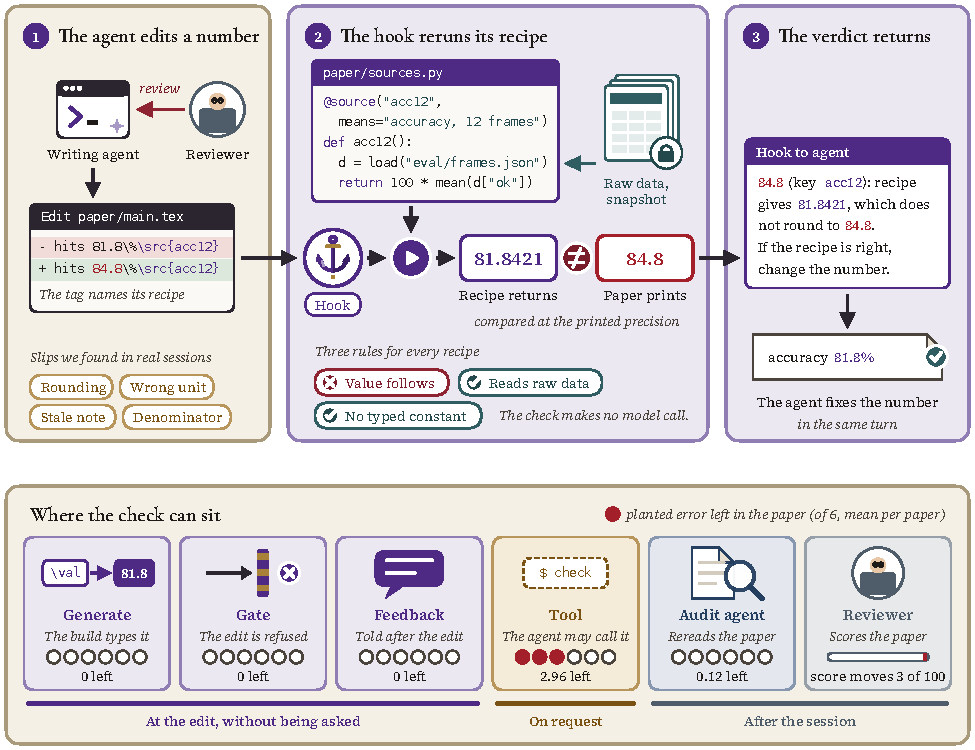
\includegraphics[width=\linewidth]{figures/fig_overview.pdf}
  \caption{\tool{} at one edit, and the six places a number check can sit. Top: (1) under a review, the writing agent
  changes a number and keeps its tag; (2) the hook finds the tag's recipe in \code{paper/sources.py}, reruns it on a
  snapshot of the repository's raw data, and compares the unrounded result with the printed number at the printed
  precision, under three rules; (3) the verdict returns to the agent, which fixes the number in the same turn. The
  cards show the content of each step for one schematic number; amber chips name the kinds of slip we found in real
  sessions (Table~\ref{tab:natural}). Bottom: the placements we compare, in session order. Dots give the measured
  mean number of planted errors left per paper, of up to six, in the placement study (Table~\ref{tab:placement});
  the reviewer's bar shows how far five wrong numbers move its score (Fig.~\ref{fig:reviewers}).}
  \label{fig:overview}
\end{figure}

\tool{} is a function from an edit to a verdict. Its inputs are the paper before and after the edit, the repository,
and a file of recipes. Its output says, for every number the edit added or changed, whether that number follows from
the repository's data, and if not, why and what value the data gives. Where this verdict goes (back to the agent, into
a denial, or into a log) is the placement, which Section~\ref{sec:placement} describes. Figure~\ref{fig:overview}
follows one number through the check.

\subsection{The recipe and the check}

Let $\mathcal{R}_0$ be a snapshot of the repository taken before the writing session starts, and let $P$ and $P'$ be
the paper's \LaTeX{} source before and after an edit. We write $\Delta(P, P')$ for the numbers that the edit inserted
or changed in place. Numbers that only moved with their text are not in $\Delta$, and neither are bare integers below
10, which are mostly counts and section numbers. A printed number $n$ has a value $v(n)$ and $d(n)$ decimals.

For each number it adds or changes, the agent writes a tag \srcmacro{} right after the number (a \LaTeX{} macro that
prints nothing) and a recipe with the same key in \code{paper/sources.py}:
\begin{lstlisting}[language=Python]
% paper/main.tex
... with 12 frames, accuracy reaches 70.4\%\src{acc12} ...

# paper/sources.py
@source("acc12", means="accuracy (%) of our model with 12 frames")
def acc12():
    d = load("eval_results/frames.json")
    xs = [v["correct"] for v in d.values() if v["num_frames"] == 12]
    return 100 * sum(xs) / len(xs)
\end{lstlisting}
The recipe $r_k$ for key $k$ returns an unrounded value, and its \code{means} string $m_k$ says in words what it
computes. The checker runs every recipe in a separate process with the repository root as working directory and
records the files $F(r_k)$ that the recipe opens.

A number passes when three rules hold.
\begin{enumerate}
  \item \textbf{The value follows.} The recipe's value must round to the printed value at the printed precision. The
        checker does the rounding, so truncation and rounding slips fail.
  \item \textbf{The recipe reads raw data.} It must open at least one file outside \code{paper/}, none of them a
        prose note (Markdown and similar formats, which go stale), and all of them present and unchanged in the
        snapshot, so an agent cannot write a data file and then cite it.
  \item \textbf{No typed constant.} The recipe may neither contain the printed value as a constant nor call a
        rounding function.
\end{enumerate}
With $\mathcal{D}_0$ the data files of $\mathcal{R}_0$ that satisfy the second rule, the check is
\begin{equation}
  \mathrm{pass}(n) \iff \bigl|\, r_k(\mathcal{R}_0) - v(n) \,\bigr| \le \tfrac{1}{2}\, 10^{-d(n)}
  \;\wedge\; \emptyset \neq F(r_k) \subseteq \mathcal{D}_0
  \;\wedge\; \neg\, \mathrm{banned}(r_k, n),
  \label{eq:pass}
\end{equation}
where $\mathrm{banned}(r_k, n)$ holds if the recipe contains $v(n)$ as a constant or calls a rounding function. The
check applies to every $n \in \Delta(P, P')$ with key $k$, with the usual unit conversions for percentages, ranges, and
K, M, and B suffixes. A number in $\Delta$ without a tag fails.

When a number fails, the message names it, gives the recipe's value, and tells the agent to first confirm that the
recipe computes what the sentence claims and, if it does, to change the number and never the recipe. For the
number of Fig.~\ref{fig:overview}, the agent reads:
\begin{card}[nwpurple]{Hook to agent (feedback mode)}
\begin{lstlisting}[style=plain]
Feedback only, your edit was kept. 1 number(s) could not be recomputed from the repository's data:
- 84.8 (line 212, key acc12): recipe gives 81.8421, which does not round to 84.8 at the printed
  precision. Context: with 12 frames, accuracy reaches 84.8\%
When a recipe disagrees with the text, first check that the recipe computes exactly what the sentence
claims; if it does, the number in the text is what must change. Never adjust a recipe just to
reproduce a printed number.
\end{lstlisting}
\end{card}

\paragraph{Why the writer writes the recipe.}
A checker that has to guess which stored value a sentence refers to must search, and Section~\ref{sec:checkers}
shows that searching fails on real repositories: they hold thousands of values, and a wrong number usually sits close
to one of them. The agent that types a number knows which computation it has in mind, so we ask it to say so. The
recipe turns an open question (does anything in this repository support this number) into a closed one (does this
computation on this data give this number), and the closed question has a deterministic answer.

\paragraph{What the check does not decide.}
The check does not decide whether a recipe computes the quantity the sentence describes. A recipe can count 14
series where the sentence means 12 distinct ones and pass. The \code{means} string records the writer's intent so that
a co-author, a reviewer, or a second model can compare it with the sentence, and Section~\ref{sec:checkers} measures
how often this gap matters.

\subsection{Where the check runs}
\label{sec:placement}

The same verdict can reach the agent in several ways. These are the placements we compare, and the bottom row of
Fig.~\ref{fig:overview} orders them along the session.

\paragraph{Tool.} The checker is available as a command, and the rules for tags and recipes are in the agent's
prompt. Nothing runs unless the agent calls it.

\paragraph{Feedback.} Claude Code lets a project run its own program before a tool call (a PreToolUse hook), after
it (PostToolUse), and when the agent is about to end its turn (Stop). After any change to the paper, whether
through an edit tool or a shell command, a PostToolUse hook runs the full check and tells the agent which numbers fail. The edit is always kept.

\paragraph{Gate.} A PreToolUse hook applies each proposed edit to \code{paper/*.tex} in memory, runs
Eq.~\eqref{eq:pass}, and denies the edit if any number fails. A shell command that changes a \code{.tex} file is
reverted, and a Stop hook refuses to let the session end while any tagged number fails, up to a fixed number of
times. The hook's state lives outside the repository, so the agent cannot edit it by accident.

\paragraph{Generate.} Instead of typing a number, the agent writes \valmacro{}, and the build replaces it with the
recipe's value rounded to $d$ decimals. The printed number cannot drift from its recipe, and the check reduces to the
second and third rules.

\paragraph{Commit.} A git pre-commit hook reruns every recipe for every tagged number and every placeholder in a
staged paper, so a recipe changed after its number was approved is caught before it reaches the shared history. This
path needs no agent and works with any editor.
